\section{SRNDeblur}
The base model, taken from the paper \cite{SRN-DeblurNet},  is the following:
\begin{figure}[H]
    \centering
    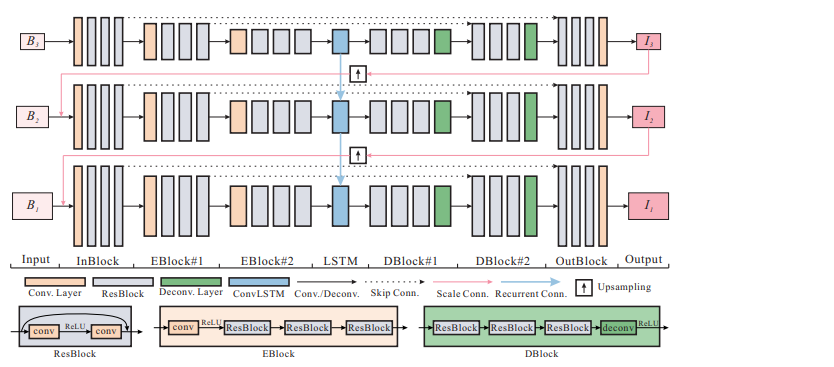
\includegraphics[scale=0.5]{subsections/srndeblur/model.png}
\end{figure}

In image deblurring an encoder-decoder network is not going to produce very sharp  results. 
In order to  improve this, \cite{SRN-DeblurNet} create a \textbf{recurrent network} which shares parameters among different \textbf{scale} thanks to residual connectivities which lead to better performance and faster training times.

The idea is that all scales are going to solve the same problem therefore they should use the same parameters.

The network takes blurred images at different scales and learn to produce sharp images at the corresponding level.
Moreover scale connection between the output in a scale and input in the next one allow the reuse of parameters within different scales and skip connections on the same level allow to improve the quality of the result as well as the training time.

A novelty introduced by \cite{SRN-DeblurNet} is the use of a \textbf{recurrent layer} which share its internal state with the recurrent layer in the next one allowing to share information that are able to improve the quality of the deblurred image.

This architecture exploit all the technique introduced in the literature up to now:
\begin{enumerate}
    \item Fully connected convolutional neural network which allows the network to handle any input (provided that the machine is able to handle the input in memory)
    \item The creation of blocks which allow to scale easily the network
    \item The encoder-decoder architecture
    \item The use of residual blocks
    \item The use of multi-scale CNN
    \item The use of a recurrent layer
\end{enumerate}

\subsection{Architecture}
The implementation of the network for both \textit{CIFAR10} and \textit{REDS} was done using only \textbf{two scales} in order to reduce the number of parameters and so to reduce the learning time.

Moreover due to the memory limitation the datasets are handled with different architectures:
\begin{center}
    \begin{minipage}[t]{0.5\textwidth}
        \textbf{CIFAR10}
        \begin{itemize}
            \item BatchNormalization is used
            \item LeakyRELU activation is used
            \item Sigmoid activation in the final layer
            \item LSTM layer is used ( In order to accommodate the input the following layers are added: 
            
            $ \textnormal{Reshape} \rightarrow \textnormal{LSTM\footnote{32 hidden units were used at each scale in order to reuse the internal state and reduce the overhead}} \rightarrow \textnormal{Dense}\footnote{Hidden units equal to the multiplication of the input dimensions ($width \times height \times channels$)} \rightarrow \textnormal{Reshape} $)
        \end{itemize}
    \end{minipage}%
    \begin{minipage}[t]{0.5\textwidth}
        \textbf{REDS}
        \begin{itemize}
            \item No BatchNormalization is used
            \item Relu activation is used
            \item No activation function is used in the final layer
            \item Conv2DLSTM layer is used 
            
            \begin{center}
                (This is the configuration used inside the paper)
            \end{center}
            
            \item Input layer is  concatenation of two layers over the filter dimension instead of a single Conv2D layer.
        \end{itemize}
        
    \end{minipage}        
\end{center}

The hyperparamters are the following:
\begin{center}
    \begin{minipage}[t]{0.5\textwidth}
        \textbf{CIFAR10}
        \begin{itemize}
            \item Filters start from 32
            \item Batch size is 150
            \item Epochs are 70
            \item Adam learning rate: $1e^{-3}$
        \end{itemize}
    \end{minipage}%
    \begin{minipage}[t]{0.5\textwidth}
        \textbf{REDS}
        \begin{itemize}
            \item Filters start from 8 (increased to 16 concatenating channels in the input in order to avoid \textit{OutOfMemory} error).
            \item Batch size is 10.
            \item Epochs are 150 ( average training time is 1h15m therefore time spent for training is 150*75=187h30m).
            \item Amount of patches extracted per image equals to 2 of size $256 \times 256$
            \item Adam learning rate: $1e^{-4}$
        \end{itemize}
    \end{minipage}        
\end{center}

\subsection{REDS Training set}

In order to cope with low memory and high training time, a tradeoff between batch size and training set size was necessary. 

\begin{enumerate}
    \item The first 24 scenes on the training set were used as validation set
    \item It's used half of the training set \footnote{It's used the following expression self.dir\_sharp.glob(**/000000[5-9][0-9].png)}
    \item Two patches are taken from each image: the idea is that the more are the patches taken the greater is the probability that patches contain a motion blur. For instance with $\textnormal{batch\_size}=10$ and $\textnormal{num\_patches}=2$ at each batch $10//2=5$ images are selected.
    \item An analysis of the training set show that the probability that a patch is too perfect [Figure \ref{high_ssim_patch1} and \ref{high_ssim_patch2}] is 29\% (using kernel density estimation\footnote{Refer to reds\_generator\_histogram\_test.py} - Figure \ref{kde_train}) therefore the \textbf{ssim} of patches extracted is computed in order to take the ones with a ssim less than $\textnormal{ssim\_threshold} = 0.9$ for avoiding patches that could influence negatively the training and so use as efficiently as possible each epoch.
    In order to maintain a generalization during the training when the threshold is not satisfied, random patches are taken.\footnote{Refer to reds\_generator.py get\_all\_patches}

    \begin{figure}[H]
        \centering
        \begin{subfigure}{0.4\textwidth}
            \centering
            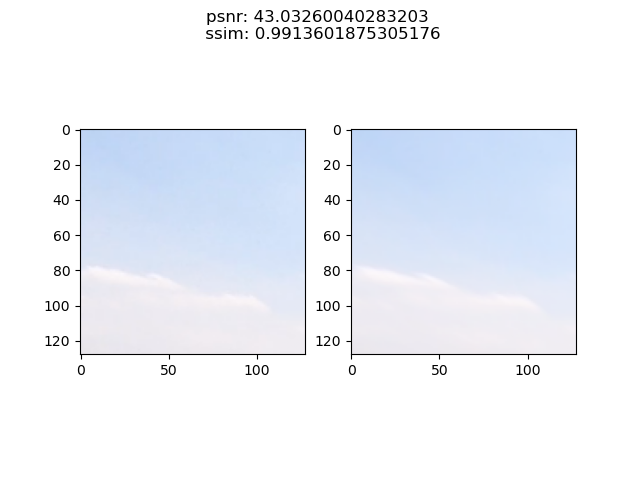
\includegraphics[scale=0.3]{subsections/srndeblur/image_sky_high_psnr.png}
            \caption{Random patch.}
            \label{high_ssim_patch1}
        \end{subfigure}
        \centering
        \begin{subfigure}{0.4\textwidth}
            \centering
            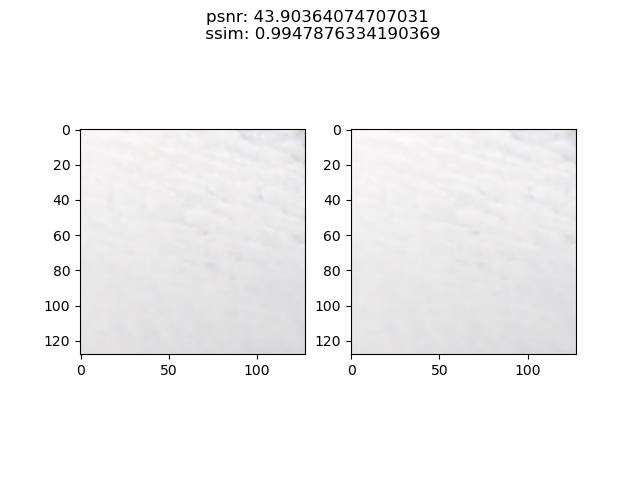
\includegraphics[scale=0.3]{subsections/srndeblur/image_sky_high_psnr.2.png}
            \caption{Random patch.}
            \label{high_ssim_patch2}
        \end{subfigure}
        \begin{subfigure}{\textwidth}
            \centering
            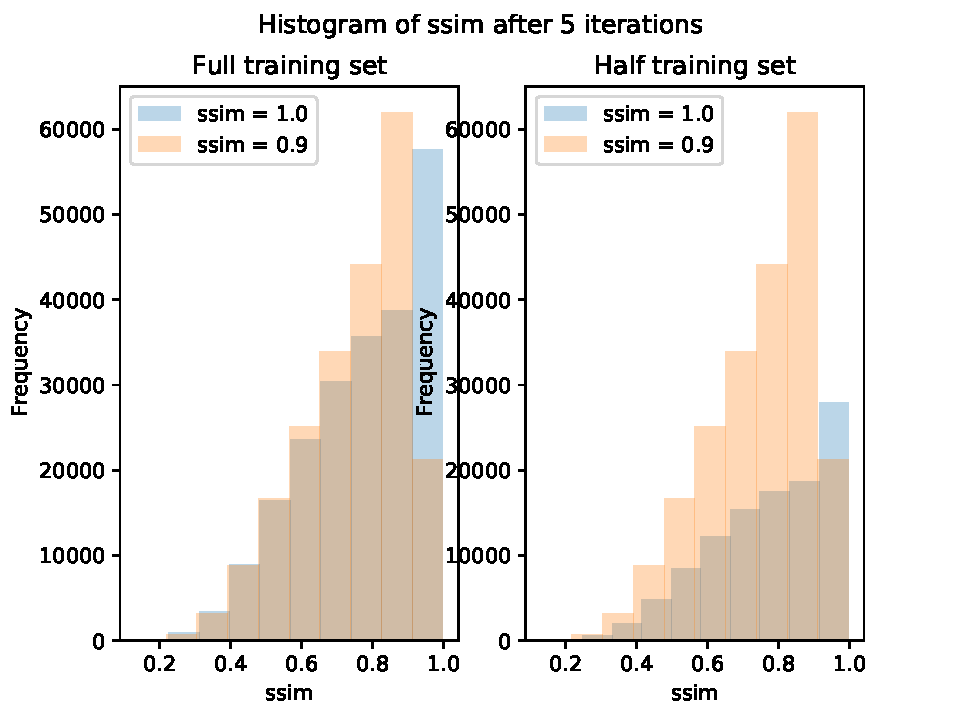
\includegraphics[width=0.3\textwidth,keepaspectratio]{subsections/srndeblur/histogram.pdf}
            \caption{Histogram of the training set}
        \end{subfigure}
        \begin{subfigure}{\textwidth}
            \centering
            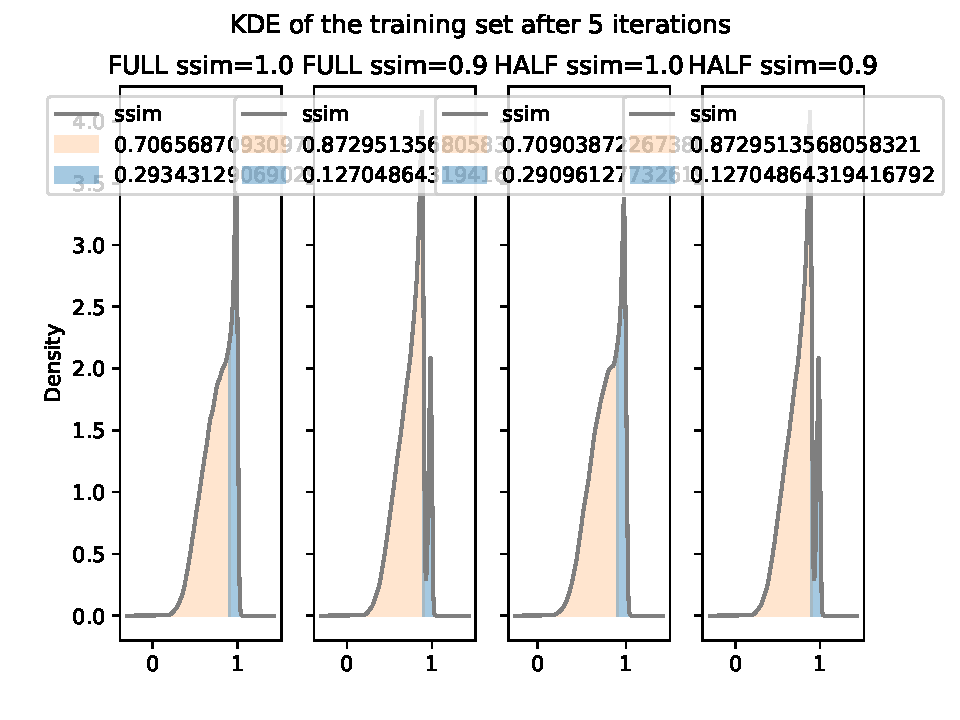
\includegraphics[width=0.6\textwidth,keepaspectratio]{subsections/srndeblur/kde.pdf}
            \caption{Kernel density estimation of the training set}
            \label{kde_train}
        \end{subfigure}
        \caption{Random patches. Histogram and kernel density estimation (using default parameters) of the full and half training set.}
    \end{figure}
\end{enumerate}

\subsection{Training}
The network was trained with Adam\cite{adam} using a learning rate of $1e^{-4}$ and MSE as loss function for both the output.
The network used is the one at the epoch 150 when the training was stopped.
Were spent 10h/day for training resuming each time the training. 
\textbf{SRNDeblur\_reds} was trained for \textbf{150 epochs in {\raisebox{0.5ex}{\texttildelow}} 180h}. SRN\-DeblurNet\cite{SRN-DeblurNet} was trained for 2000 epochs in 72h. 

\begin{figure}[H]
    \centering
    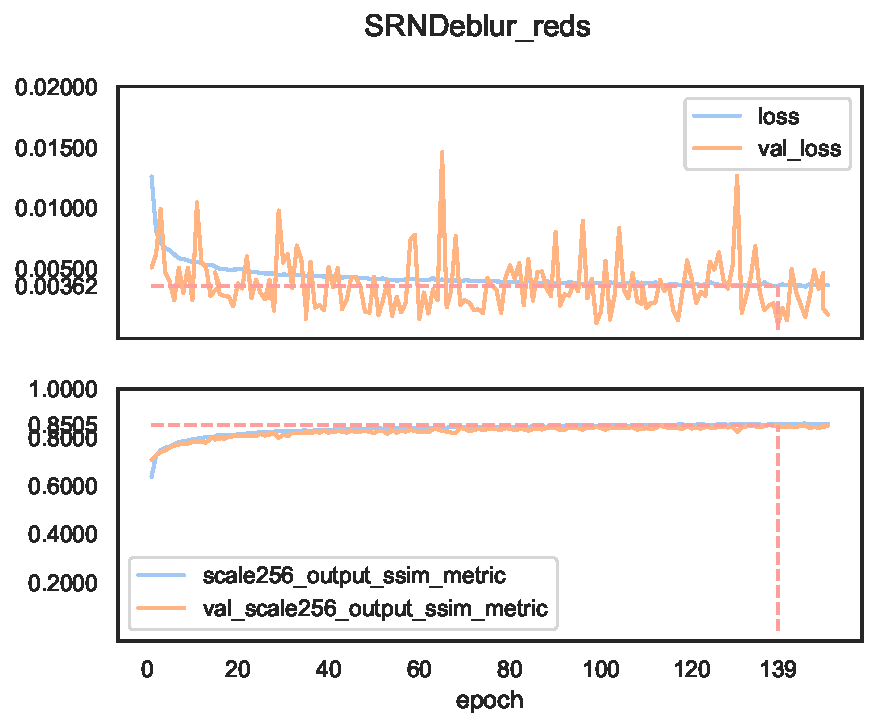
\includegraphics[scale=0.35]{subsections/srndeblur/plot_history_SRNDeblur_reds.pdf}
    \caption{Training information SRNDeblur\_reds}
\end{figure}

Different from the paper, the learning rate was not reduced to $1e^{-6}$ over 2000 epochs with an exponential decay, because  I have thought to stop at 150 epochs since the beginning; this is, probably, the cause of the plateau of the loss.

\section{Results}
The evaluations are the following:

\begin{tabularx}{300pt}{cccc}
            CIFAR10 network & MSE & PSNR & SSIM \\
            \hline
            \textnormal{Without LSTM} & 0.00175 & 29.23 & 0.9225 \\
            \textnormal{With LSTM} & 0.00174 & 29.38 & 0.9188 \\
            \hline
\end{tabularx}

\begin{tabularx}{300pt}{cccccc}
            & \multicolumn{3}{c}{SRNDeblur\_reds\footnote{The evaluation is done deblurring full hig res images and then computing their ssim. The average evaluation over 500 samples is returned.}} & \multicolumn{2}{c}{SRN-DeblurNet} \\
dataset & MSE & PSNR & SSIM & PSNR & SSIM \\
\hline
REDS & 0.002 & 27.23 & 0.8105 & - & - \\
GOPro & - & - & - & 30.26 & 0.9342 \\
\hline            
\end{tabularx}            
\begin{figure}[H]
    \centering
    \begin{subfigure}{\textwidth}
        \centering
        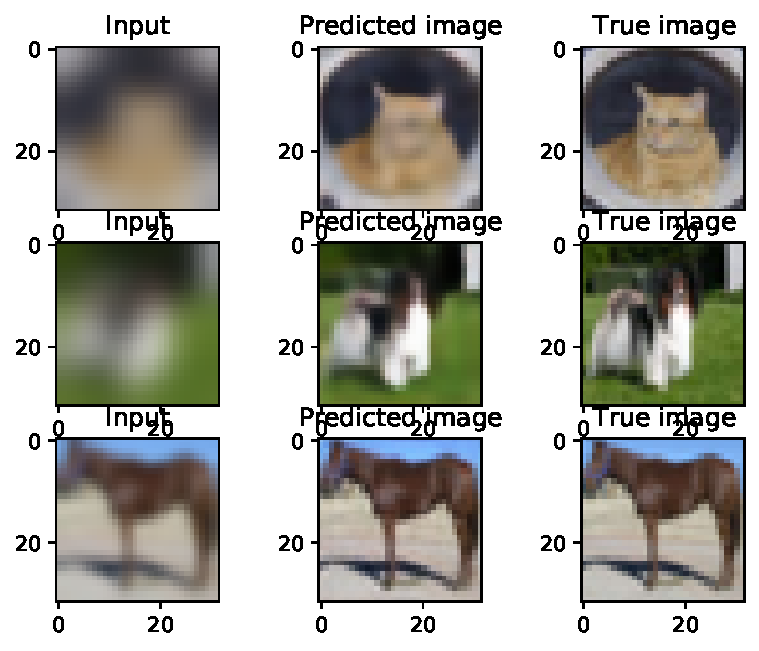
\includegraphics[height=0.48\textheight]{subsections/srndeblur/cifarnolstmtest.pdf}
        \caption{Test image generated by SRNDeblur\_cifar network without LSTM }
    \end{subfigure} 
    \begin{subfigure}{\textwidth}
        \centering
        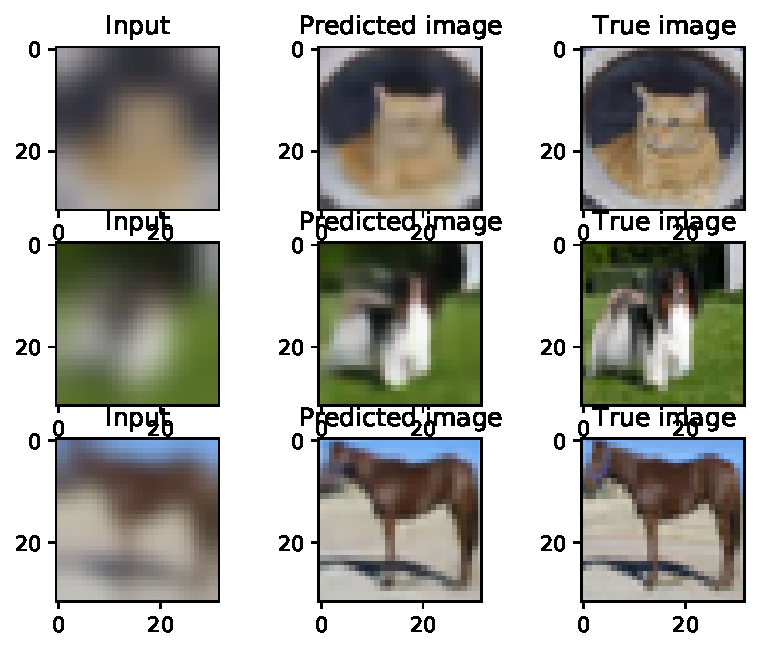
\includegraphics[height=0.48\textheight]{subsections/srndeblur/cifarlstmtest.pdf}
        \caption{Test image generated by SRNDeblur\_cifar network with LSTM }
    \end{subfigure} 
\end{figure}

\begin{figure}[H]
    \centering
    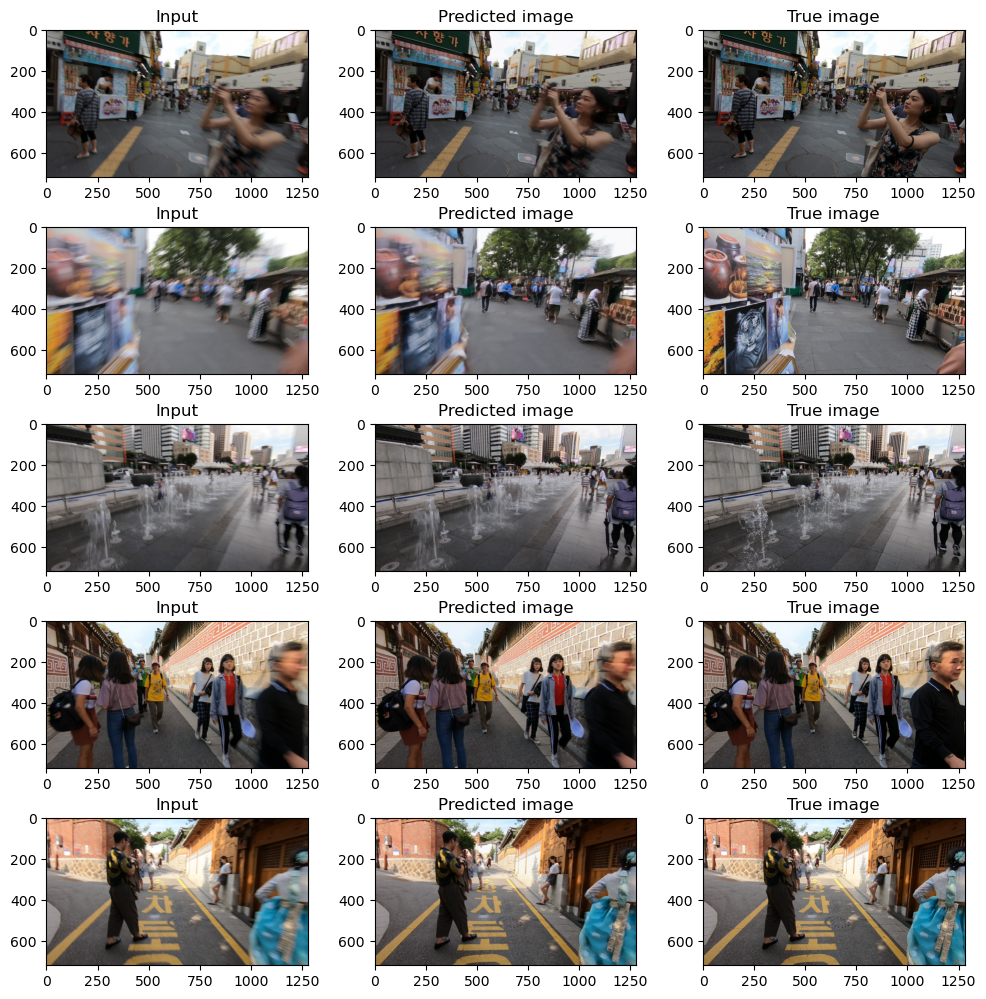
\includegraphics[width=\textwidth,keepaspectratio]{subsections/srndeblur/test.png}
    \caption{Test image on high resolution test set generated by REDS network.}
\end{figure}

\begin{figure}[H]
    \centering
    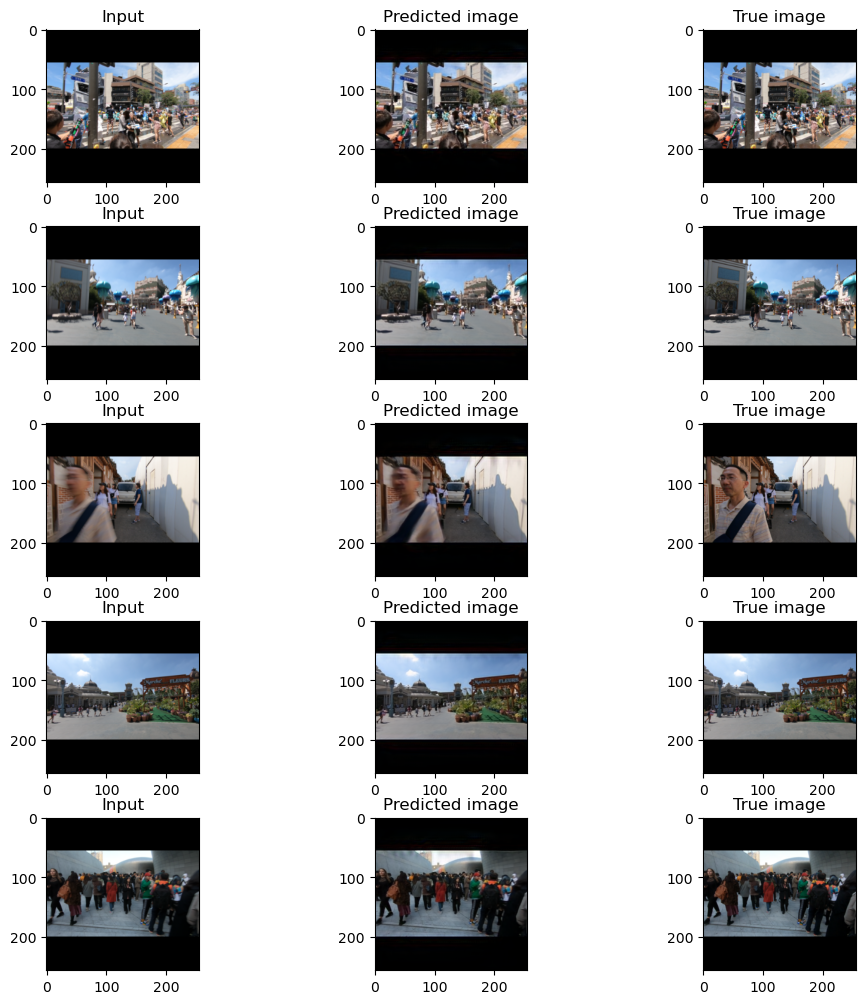
\includegraphics[width=\textwidth,keepaspectratio]{subsections/srndeblur/test.low_res.png}
    \caption{Test image on low resolution test set generated by REDS network.}
\end{figure}
